\section{Recovering SGDM with Online Mirror Descent}
\label{sec:Exp-O2NC_sgdm}

In the previous sections, we have shown that Exponentiated O2NC can convert any OCO algorithm into a non-convex optimization algorithm in such a way that small regret bounds transform into convergence guarantees. So, the natural next step is to instantiate \alg\ with some particular OCO algorithm. In this section we carry out this task and discover that the resulting method not only achieves optimal convergence guarantees, but is also \emph{nearly identical} to the standard SGDM optimization algorithm!

The OCO algorithm we will use to instantiate Exponentiated O2NC is a simple variant of ``online mirror descent'' (OMD) \cite{beck2003mirror}, which a standard OCO algorithm. However, typical OMD analysis involves clipping the outputs $\Delta_n$ to lie in some pre-specified constraint set. We instead employ a minor modification to the standard algorithm to obviate the need for such clipping. 
% This algorithm works for any arbitrary sequence of gradients $\tilde\vecg_t$ for $t=1,\ldots,n$. In the context of Exponentiated O2NC, $\tilde\vecg_t = \beta^{-t}\vecg_t$.

Inspired by \cite{duchi2010composite}, we choose our OCO algorithm from the family of Online Mirror Descent (OMD) with composite loss.  Given a sequence of gradients $\tilde\vecg_t:=\beta^{-t} \vecg_t$ and convex functions $\psi_t(\Delta), \calR_t(\Delta), \phi_t(\Delta)$, OMD with composite loss defines $\Delta_{t+1}$ as:
\begin{equation*}
    % \Delta_{t+1} = 
    \argmin_\Delta \langle\tilde\vecg_t, \Delta\rangle + D_{\psi_t}(\Delta,\Delta_t) + \underbrace{\calR_{t+1}(\Delta) + \phi_t(\Delta)}_{\text{composite loss}}.
    \label{eq:Exp-O2NC:omd-update}
\end{equation*}
Here $D_{\psi_t}$ denotes the Bregman divergence of $\psi_t$, and $\calR_{t+1}(\Delta)+\phi_t(\Delta)$ denotes the composite loss. 
% Without $\phi_t$, this update formula simplifies back to the conventional OMD update. The introduction of composite loss serves as a counterbalance to the potentially large norms of $\Delta_t$, effectively acting as a norm regularizer. 
The composite loss consists of two components. Firstly, $\calR_{t+1}(\Delta)=\frac{\mu_{t+1}}{2}\|\Delta\|^2$ controls the variance of $\vecy_n$, as discussed in Section \ref{sec:Exp-O2NC_alg}. Secondly, OMD is known to struggle under unconstrained domain setting \cite{orabona2016scale}, but this can be fixed with proper regularization, as done in \citet{fang2021online} (implicitly), and \citet{jacobsen2022parameter} (explicitly). Following a similar approach, we set $\phi_t(\Delta)=(\frac{1}{\eta_{t+1}}-\frac{1}{\eta_t})\|\Delta\|^2$ to prevent the norm of $\|\Delta\|$ from being too large.

% In particular, we choose $\psi_t(\Delta) = \frac{1}{2\eta_t}\|\Delta\|^2$ where $\eta_t$ denotes some learning rate such that $0<\eta_{t+1}\le \eta_t$. Moreover, with slight abuse of notation, we define the composite loss as $\calR_{t+1}(\Delta) + \phi_t(\Delta)$. Here $\calR_{t+1}(\Delta)=\frac{\mu_{t+1}}{2}\|\Delta\|^2$ functions as the variance regularizer of \alg (as detailed in Section \ref{sec:Exp-O2NC_alg-design}); $\phi_t(\Delta)=(\frac{1}{\eta_{t+1}}-\frac{1}{\eta_t})\|\Delta\|^2$ serves as the norm regularizer for the unconstrained domain.


With $\psi_t(\Delta) = \frac{1}{2\eta_t}\|\Delta\|^2$ where $0<\eta_{t+1}\le \eta_t$, Theorem \ref{thm:Exp-O2NC:OGD-brief} provides a regret bound for this specific OCO algorithm.

\begin{theorem}
\label{thm:Exp-O2NC:OGD-brief}
Let $\Delta_1=0$ and $\Delta_{t+1} = \argmin_\Delta \langle\tilde\vecg_t,\Delta\rangle + \frac{1}{2\eta_t}\|\Delta-\Delta_t\|^2 + \frac{\mu_{t+1}}{2}\|\Delta\|^2 + (\frac{1}{\eta_{t+1}}-\frac{1}{\eta_t})\|\Delta\|^2$. Then
\begin{align*}
    &\sum_{t=1}^n \langle \tilde\vecg_t, \Delta_t-\vecu\rangle + \calR_t(\Delta_t) - \calR_t(\vecu) \\
    &\le \left(\frac{2}{\eta_{n+1}} + \frac{\mu_{n+1}}{2}\right)\|\vecu\|^2 + \frac{1}{2}\sum_{t=1}^n \eta_t\|\tilde\vecg_t\|^2.
\end{align*}
\end{theorem}

% Before we draw connections with \alg, we'd like to highlight some key takeaways from Theorem \ref{thm:Exp-O2NC:OGD-brief}. 
Note that the implicit OMD update described in Theorem \ref{thm:Exp-O2NC:OGD-brief} can be explicitly represented as follows:
\begin{equation}
    \Delta_{t+1} = \frac{\Delta_t-\eta_t\tilde\vecg_t}{1+\eta_t\mu_{t+1}+\eta_t(\frac{1}{\eta_{t+1}}-\frac{1}{\eta_t})}.
    \label{eq:Exp-O2NC:ogd-explicit}
\end{equation}
When $\calR_t=0$ (implying $\mu_t=0$), the update formula in \eqref{eq:Exp-O2NC:ogd-explicit} simplifies to an approximation of \emph{online gradient descent} \cite{zinkevich2003online}, albeit with an additional scaling.
% In other words, Theorem \ref{thm:Exp-O2NC:OGD-brief} gives a regret bound of an unconstrained variant of online gradient descent with varying step-size.


\subsection{Reduction of \alg}

Upon substituting $\tilde\vecg_t = \beta^{-t}\vecg_t$ where $\vecg_t=\nabla f(\vecx_t,z_t)$, Theorem \ref{thm:Exp-O2NC:OGD-brief} provides a regret bound for $\regret_n(\vecu_n)$ in the convergence bound in Theorem \ref{thm:Exp-O2NC:o2nc}. Consequently, we can bound $\E\|\nabla F(\overline\vecx)\|_c$ for \alg with the unconstrained variant of OMD as the OCO subroutine (with update formula described in \eqref{eq:Exp-O2NC:ogd-explicit}). Formally, we have the following result:

\begin{restatable}{theorem}{SGDM}
\label{thm:Exp-O2NC:sgdm}
Follow Assumption \ref{as:Exp-O2NC:optimization} and consider any $c>0$. Let $\Delta_1=0$ and update $\Delta_t$ by
\begin{equation*}
    \Delta_{t+1} = \frac{\Delta_t - \eta_t\beta^{-t}\vecg_t}{1+\eta_t\mu_{t+1}+\eta_t(\frac{1}{\eta_{t+1}}-\frac{1}{\eta_t})}.
\end{equation*}
Let $\mu_t=\beta^{-t}\mu$, $\eta_t=\beta^t\eta$, $\beta=1-\alpha$, $\mu=\frac{24F^*c}{(G+\sigma)\alpha^{5/2}N}$, $\eta=\frac{2F^*}{(G+\sigma)^2N}$, $\alpha=\max\{N^{-2/3}, \frac{(F^*)^{4/7}c^{2/7}}{(G+\sigma)^{6/7}N^{4/7}}\}$. Then for $N$ large enough such that $\alpha \le \frac{1}{2}$,
\begin{align*}
    \E\|\nabla F(\overline\vecx)\|_c
    &\lesssim \frac{G+\sigma}{N^{1/3}} + \frac{(F^*)^{2/7}(G+\sigma)^{4/7}c^{1/7}}{N^{2/7}}.
\end{align*}
\end{restatable}

As an immediate implication, upon solving $\E\|\nabla F(\overline\vecx)\|_c \le \epsilon$ for $N$, we conclude that Algorithm \ref{alg:Exp-O2NC:O2NC-exp-avg} instantiated with unconstrained OGD finds $(c,\epsilon)$-stationary point within $N=O(\max\{(G+\sigma)^3\epsilon^{-3}, F^*(G+\sigma)^2c^{1/2}\epsilon^{-7/2}\})$ iterations. 
% When $c\ge\epsilon$. 
Moreover, in Section \ref{sec:Exp-O2NC_lower} we will show that this rate is optimal.

Furthermore, as discussed in Section \ref{sec:Exp-O2NC_pre}, with $c=O(\epsilon^{-1})$, this algorithm achieves the optimal rate of $O(\epsilon^{-4})$ when $F$ is smooth; with $c=O(1)$, this algorithm also achieves the optimal rate of $O(\epsilon^{-7/2})$ when $F$ is second-order smooth. Remarkably, these optimal rates automatically follows from the reduction from $(c,\epsilon)$-stationary point to $\epsilon$-stationary point (see Lemma \ref{lem:Exp-O2NC:criterion-reduction}), and neither the algorithm nor the analysis is modified to achieve these rates.
% with $c=\epsilon/\delta^2$, the definition of $(c,\epsilon)$-stationary point is a relaxation of the standard $(\delta,\epsilon)$ Goldstein stationary point.
% by relaxing a deterministic constraint, $\|\vecy_n-\overline\vecx_n\| \le \delta$, to a probabilistic one, $\E\|\vecy_n-\overline\vecx_n\|^2 \le \delta^2$. 
% Moreover, we can reduce $(c,\epsilon)$-stationary point to $\epsilon$-stationary point by setting $\delta=O(\epsilon)$ when the loss is smooth or $\delta=O(\sqrt{\epsilon})$ when the loss is second-order smooth.
% Consequently, upon substituting $c=\epsilon/\delta^2$ into Theorem \ref{thm:Exp-O2NC:sgdm}, $\E\|\nabla F(\overline\vecx)\|_c \le \epsilon$ with $N\gtrsim \max\{\frac{(G+\sigma)^3}{\epsilon^3}, \frac{F^*(G+\sigma)^2}{\delta\epsilon^3}\}$. In the scenario where $\delta=O(1)$, this oracle complexity matches the optimal rate achieved by standard O2NC \cite{cutkosky2023optimal} under the $(\delta,\epsilon)$ Goldstein stationary point criterion. Moreover, upon substituting $\delta=O(\epsilon)$, we attain the optimal rate $O(\epsilon^{-4})$ for smooth losses; similarly, with $\delta=O(\sqrt{\epsilon})$, we attain the optimal rate $O(\epsilon^{7/2})$ for second-order smooth losses.

\subsection{Unraveling the update to discover SGDM}
Furthermore, upon substituting the definition of $\eta_t,\mu_t$ (and neglecting constants $G,\sigma,F^*$), the update in Theorem \ref{thm:Exp-O2NC:sgdm} can be rewritten as
\begin{equation*}
    \Delta_{t+1} = \frac{\Delta_t - \eta\vecg_t}{1 + \frac{1}{\beta}(\eta\mu + \alpha)}
\end{equation*}
Let $\Delta_t = -\frac{\beta\eta}{\eta\mu+\alpha}\vecm_t$, then we can rewrite the update of \alg \ with OGD as follows:
\begin{align}
    &\vecm_{t+1} = \frac{\beta}{1+\eta\mu} \vecm_t + \frac{\alpha + \eta\mu}{1+\eta\mu} \vecg_t, \notag\\
    &\vecx_{t+1} = \vecx_t - s_{n+1}\cdot \frac{\beta\eta}{\eta\mu+\alpha} \vecm_{t+1}.
    \label{eq:Exp-O2NC:sgdm-1}
\end{align}
Remarkably, this update formula recovers the standard SGDM update, with the slight modification of an additional exponential random variable $s_{n+1}$: let $\tilde\beta = \frac{\beta}{1+\eta\mu}$, which denotes the effective momentum constant, and let $\tilde\eta = \frac{\beta\eta}{\eta\mu+\alpha}$ be the effective learning rate, then \eqref{eq:Exp-O2NC:sgdm-1} becomes
\begin{align}
    &\vecm_{t+1} = \tilde\beta \vecm_t + (1-\tilde\beta)\vecg_t, \notag\\
    &\vecx_{t+1} = \vecx_t - s_{t+1}\cdot \tilde\eta \vecm_{t+1}.
    \label{eq:Exp-O2NC:sgdm-2}
\end{align}

\paragraph{Smooth case}
As discussed earlier, when $F$ is smooth, we set $c=O(\epsilon^{-1})$ to recover the optimal rate $N=O(\epsilon^{-4})$. This implies $c=O(N^{1/4})$. Consequently, we can check the parameters defined in Theorem \ref{thm:Exp-O2NC:sgdm} have order $\alpha = O(N^{-1/2})$, $\eta = O(N^{-1})$, and $\mu=O(N^{1/2})$ (note that $\eta\mu\approx \alpha$). Therefore, the effective momentum constant is roughly $\tilde\beta \approx 1-\frac{1}{\sqrt{N}}$, and the effective learning rate is roughly $\tilde\eta\approx \frac{1}{\sqrt{N}}$. Interestingly, these values align with prior works \cite{cutkosky2020momentum}.

\begin{figure*}[ht]
    \vskip 0.2in
    \centering
    \begin{subfigure}[b]{0.3\linewidth}
        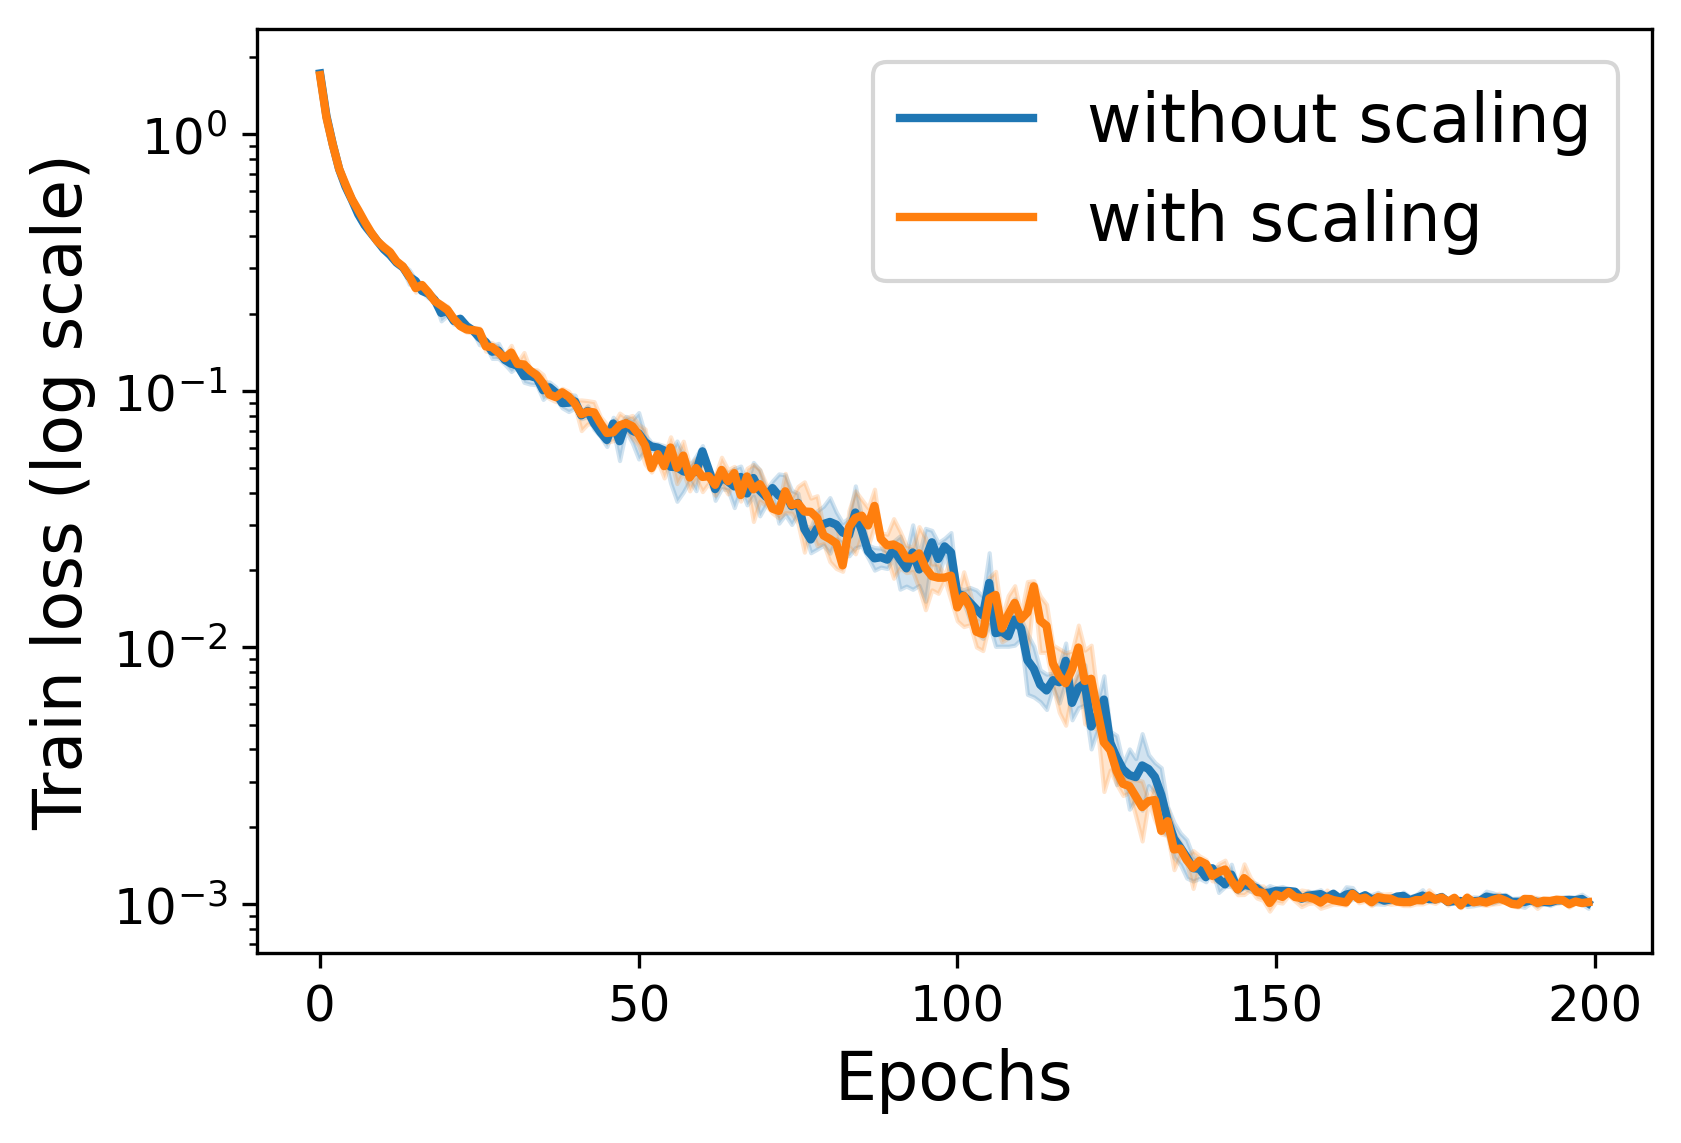
\includegraphics[width=\linewidth]{4_Exp-O2NC/img/train_loss.png}
        \caption{Train Loss}
        \label{fig:Exp-O2NC:1a}
    \end{subfigure}
    \hfill % Optional: add some horizontal spacing
    \begin{subfigure}[b]{0.3\linewidth}
        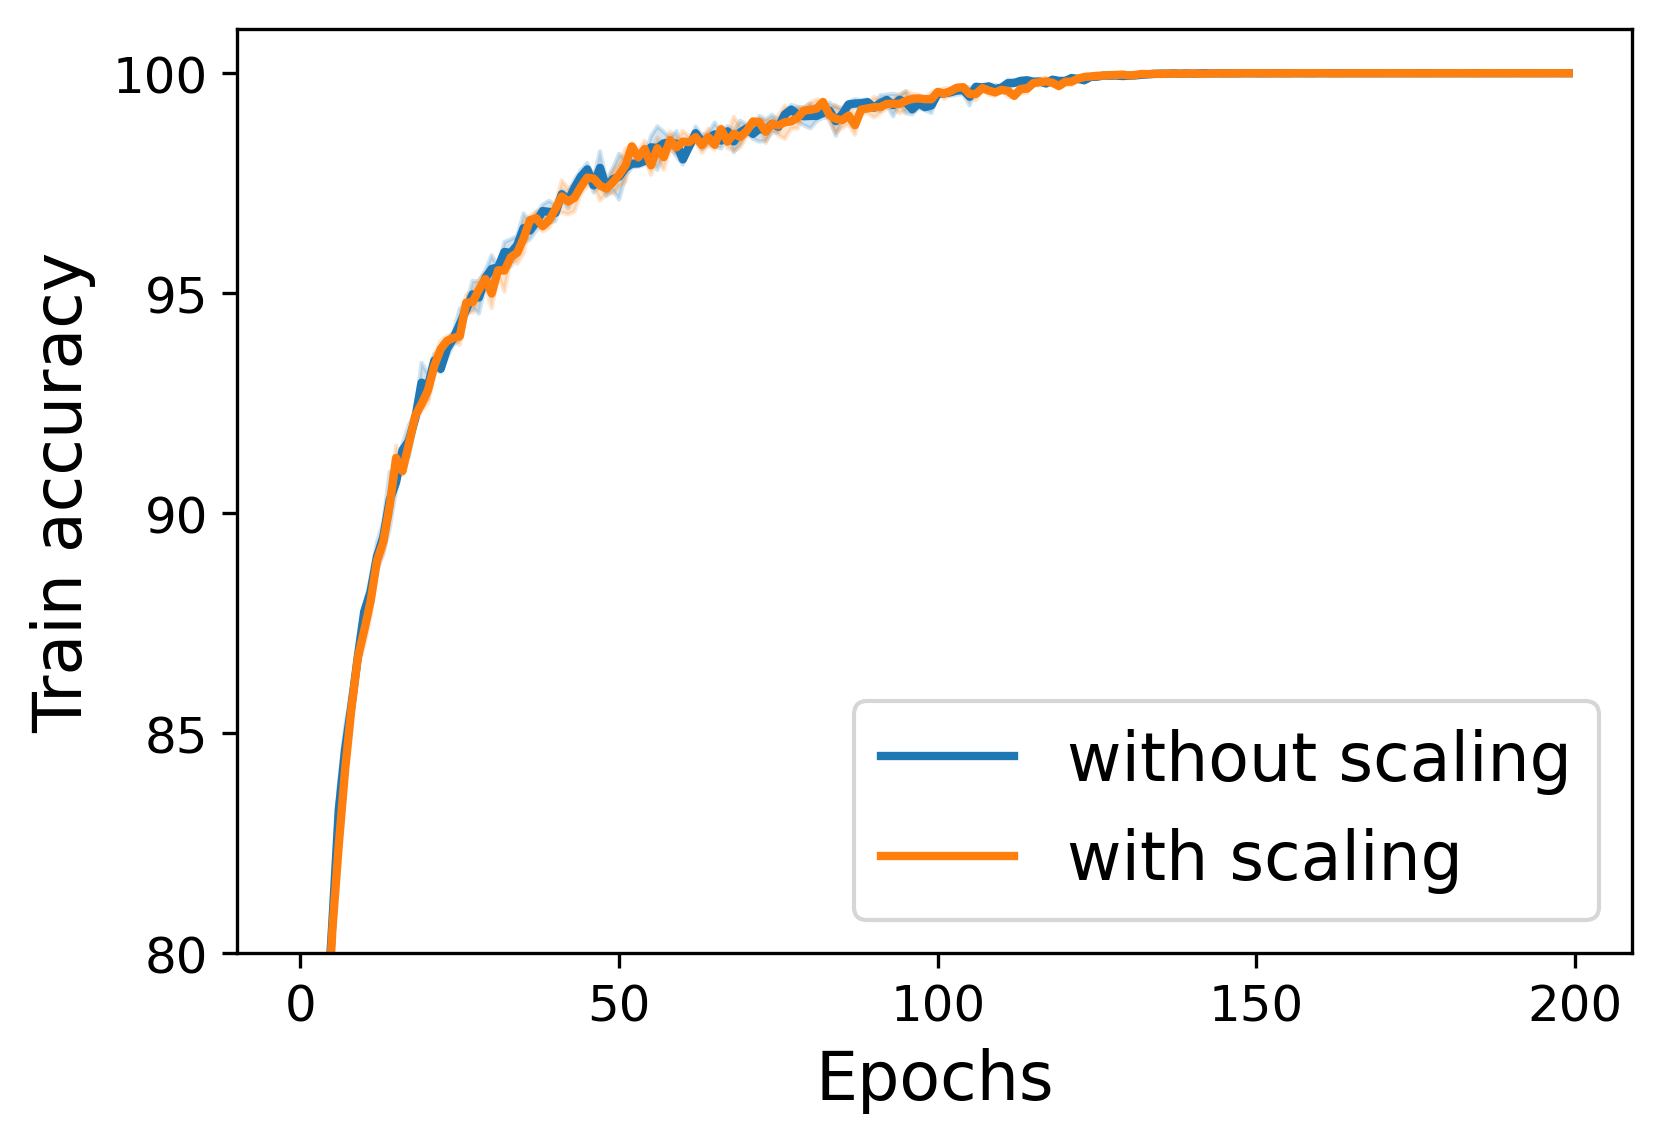
\includegraphics[width=\linewidth]{4_Exp-O2NC/img/train_acc.png}
        \caption{Train Accuracy}
        \label{fig:Exp-O2NC:1b}
    \end{subfigure}
    \hfill % Optional: add some horizontal spacing
    \begin{subfigure}[b]{0.3\linewidth}
        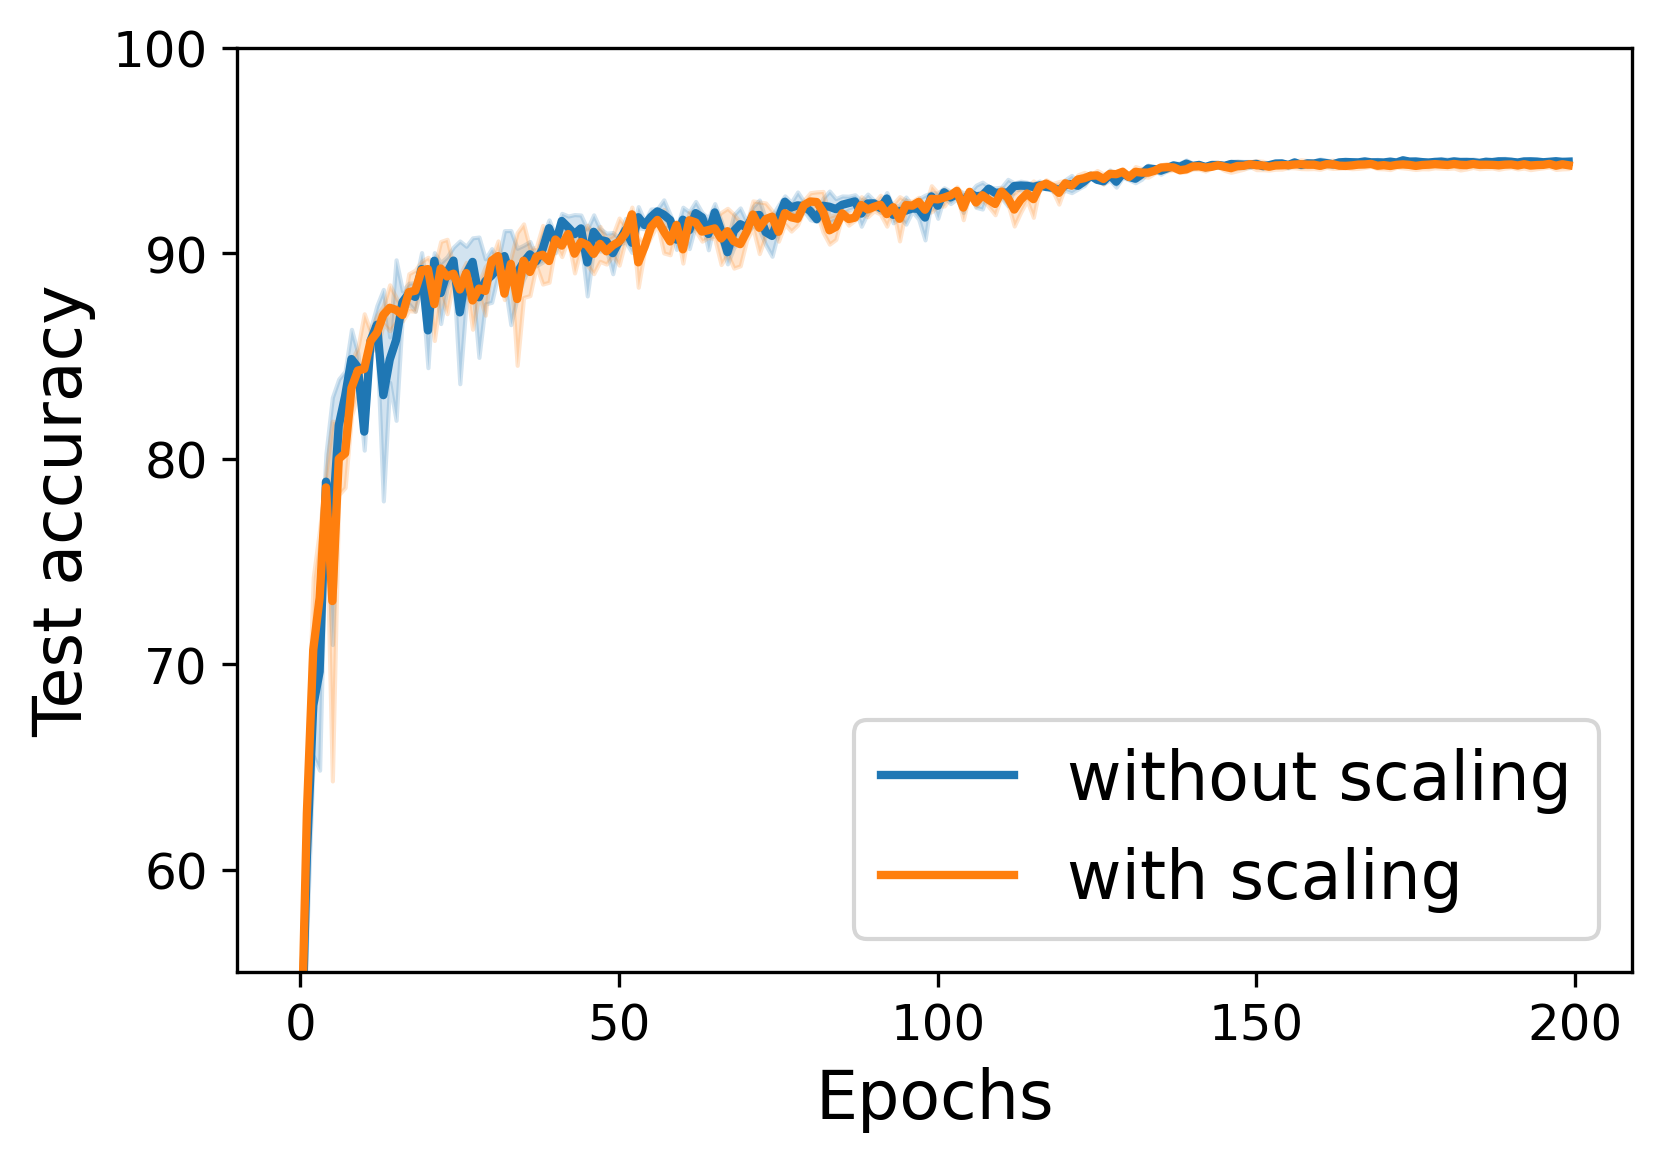
\includegraphics[width=\linewidth]{4_Exp-O2NC/img/test_acc.png}
        \caption{Test Accuracy}
        \label{fig:Exp-O2NC:1c}
    \end{subfigure}
    \caption{Experiments on CIFAR-10 with ResNet-18 Network. The curves represent the average performance of each optimizer in three trials, and the shaded regions denote the standard deviation.}
    \label{fig:Exp-O2NC:experiment}
    \vskip 0.2in
\end{figure*}

\paragraph{Second-order smooth case}
When $F$ is second-order smooth and we set $c=O(1)$, we can check that $\alpha = O(N^{-4/7})$, $\eta=O(N^{-1})$, and $\mu=O(N^{3/7})$ (again $\eta\mu\approx \alpha$). Consequently, the effective momentum should be set to $\tilde\beta \approx 1-\frac{1}{N^{4/7}}$ and the effective learning rate should be $\tilde\eta \approx \frac{1}{N^{3/7}}$. It is interesting to note that in both smooth and second-order smooth cases, $(1-\tilde\beta)\tilde\eta \approx \frac{1}{N}$.